% [FILENAME]
% Author: [AUTHOR]
% Created: [DATE]
% Updated: [DATE]
% Description: [DESCRIPTION]

% This part is used for https://github.com/hussein-esmail7/template-maker
% templateDescription: 8 - TikZ Whiteboard Template

% This file can be found at https://github.com/hussein-esmail7/templates

% =========================== Variables ===========================
\def\myAuthor			{[AUTHOR]} % Author of this file
\def\mySubject			{PDF Subject Here}  % Used for Metadata
\def\myKeywords			{PDF Keywords Here} % Separated by comma
\def\myDateUpdated		{\today}
\def\myTitle			{[FILE FRONT]}
% =========================== Variables ===========================

% =========================== Shortcuts ===========================
% =========================== Shortcuts ===========================

\documentclass{article}

\usepackage[margin=1in]{geometry} % 1-inch margins
\usepackage{comment}	% Used for the 'comment' environment (multi-line)
\usepackage{float}		% Used for ``H'' flag in figure environment
\usepackage{graphicx}   % Used for adding images
\usepackage{tikz}
\usepackage{xcolor}

\usepackage{hyperref}   % Used for adding PDF metadata

\graphicspath{{./}}     % Import images in the same folder as this .tex file

\title{\myTitle}
\author{\myAuthor}

\begin{document}			% Official beginning of the document.
\pagenumbering{gobble}		% No page numbers

\begin{figure}[h!]
	\centering
	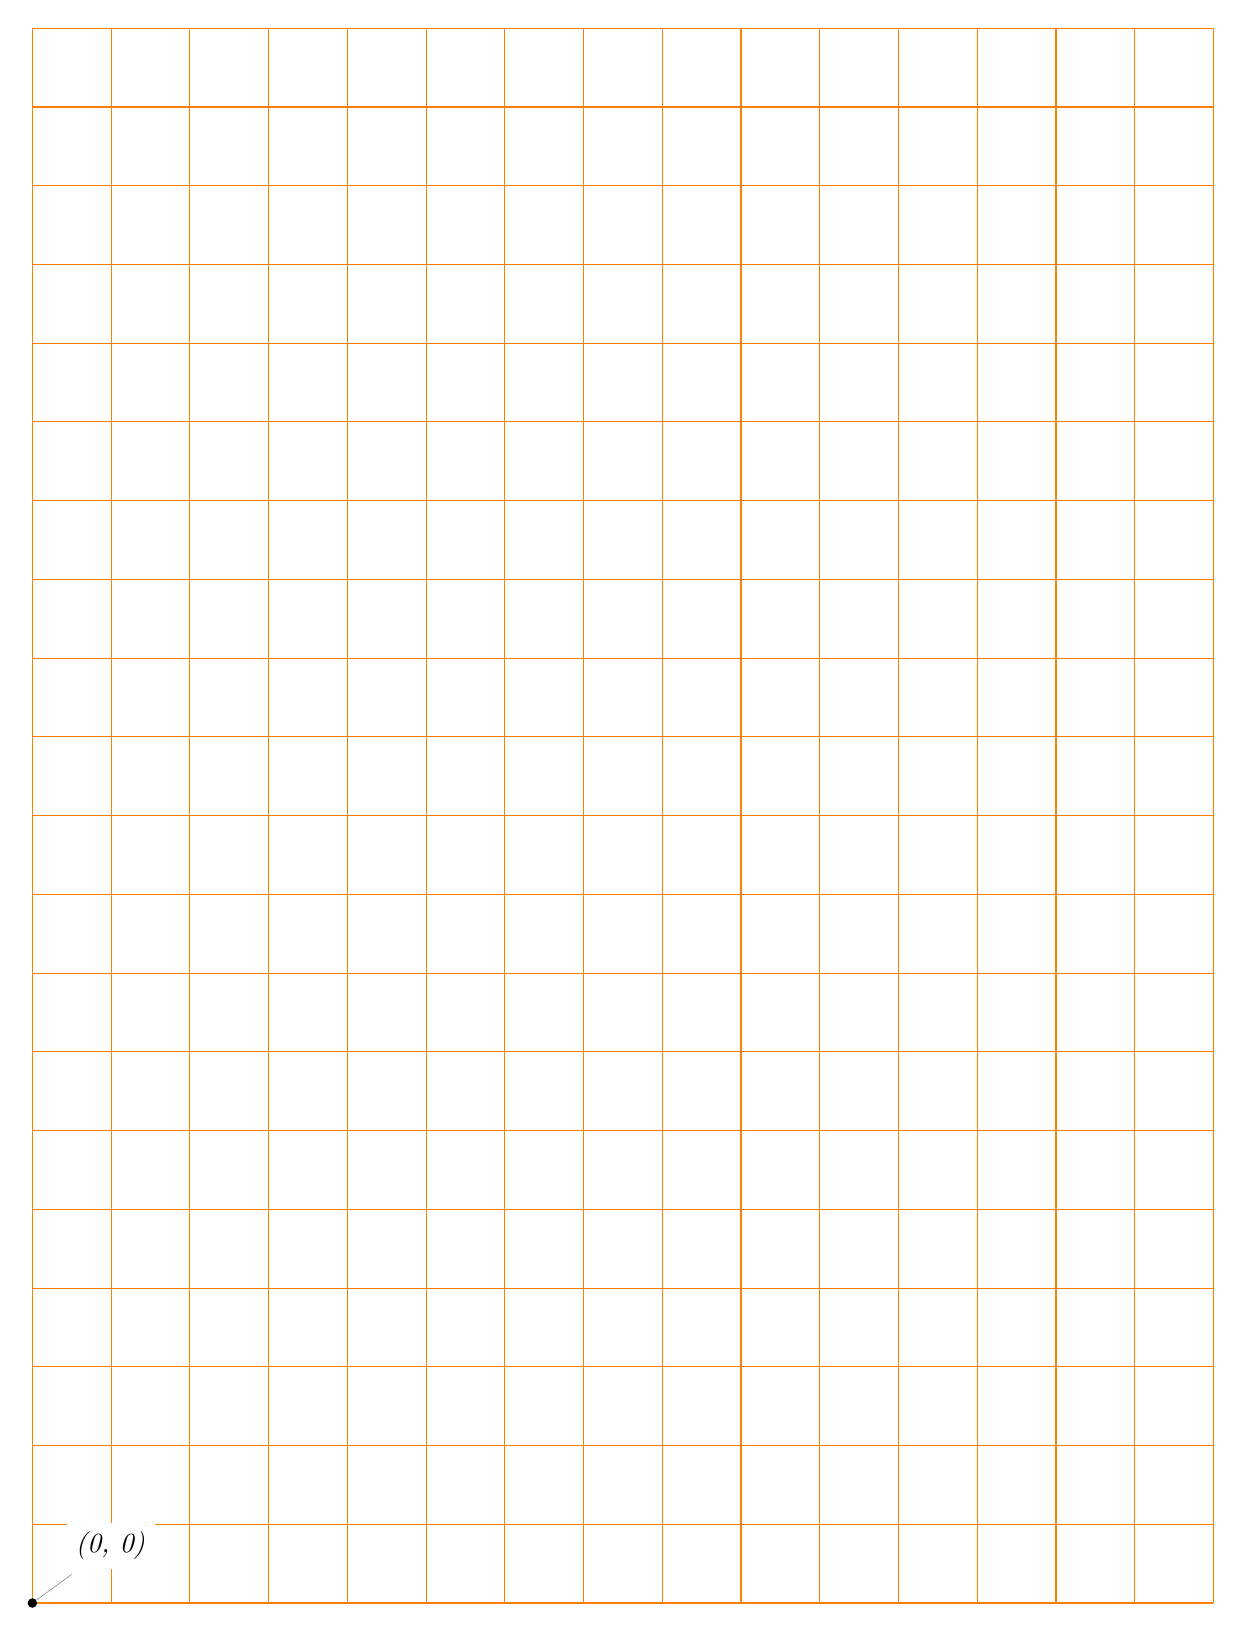
\begin{tikzpicture}
		\draw[orange] (0,0) grid[xstep=1, ystep=1]  (15, 20); % Grid
		\node [fill, draw, circle, minimum width=3pt, inner sep=0pt, pin={[fill=white, outer sep=2pt]45:\textit{(0, 0)}}] at (0,0) {}; % Pinlabel for (0, 0)
		% TODO: Remaining drawing code here
	\end{tikzpicture}
\end{figure}

\end{document}
